\chapter{Outline of baryogenesis}
One way to describe the observed baryonic asymmetry is by assuming that the universe has been in an asymmetric state just from the beginning and that the matter and antimatter is concentrated in big domains throughout the universe, which come into contact just at their outer borders. Techincally, there is no reason for the universe not to have started in an asymmetric state, but in that case one would measure high gamma rates due to the matter-antimatter-annihilation right between these distinct regions. \newline\indent \indent
Since there is no such radiation observed, patches of different kinds of matter have to be as big as the presently observable universe. Because this doesn't seem very plausible, the baryonic asymmetry had to arise dynamically from an universe where matter and antimatter existed in the same amount. \newline\indent
Actually, in 1967 Andrei Sakharov postulated the criteria, which have to be met in order for an excess of baryons over anti-baryons to be generated out of a fully symmetrical universe.
\section{Sakharov Conditions}
As mentioned above, there are three crucial properties of nature, the Sakharov conditions, which are required to produce a net baryon number greater than zero. These three conditions are:
\begin{enumerate}
	\item B-violating process(es)
	\item C and CP violation
	\item Departure from or loss of thermal equilibrium
\end{enumerate}
For a general insight into these three conditions the first one will be skipped, since it is quite obvious that in a totally symmetric universe there has to be at least one B-violating process in order to cause an imbalance in matter and antimatter. The general importance of the other two will be discussed in the following.
\subsection{C and CP-violation}
Charge conjugation (C), parity (P) and their combination (CP) are two or more specifically three basic symmetries of the universe. C symmetry states that physical processes are the same, even after exchanging particles for their respective anti-particles, while P-symmetry guarantees invariance under the transformation $\vec{r}\rightarrow-\vec{r}$. CP symmetry then simply is a sequence of a C followed by a P transformation. \newline\indent \indent
To explain both C and CP have to be violated for baryogenesis beeing possible, one has to keep in mind that any state consisting baryon number carrying particles changes the sign of its baryon number under C- as well as under CP-transformations\cite[p. 4]{Petropoulos:2003pm} This means that the only C and CP invariant states are the ones with a zero baryon number, just like our assumed initially symmetrical universe.
This implies that the baryon number in the universe stays zero, unless C and CP are violated\cite[p. 4]{Petropoulos:2003pm}. \newline \indent
\subsection{Departure from thermal equilibrium}
The last condition to be met in order for baryogenesis to be achievable is that the the B, C and CP violating processes must occur outside the thermal equilibrium. To illustrate this we first consider the thermal distribution of a species X of quantum particles
\begin{equation}
	f(E_X)=\frac{1}{e^{\frac{E_X-\mu_X}{T}}\pm1}.
	\label{eq:distribution}
\end{equation}
The energy $E_X$ and the momentum $\vec{p}_X$ are related via the relativistic energy-momentum-relation $E_X^2=\vec{p}_X^2+m_X^2$. $\mu_X$ describes the chemical potential of the particle species X, which is an important quantity for describing thermal equilibrium states, as the chemical potentials of two species X and Y, which are in thermal equilibrium, are related by $\mu_X=\mu_Y$ or for more species $\sum_i\mu_i=0$.\newline\indent
Using eq. \eqref{eq:distribution} to compute the particle density of a certain particle species one gets 
\begin{equation}
	n_X=g_X\int\frac{d^3p}{(2\pi)^3}\:f_X(E),
	\label{eq:density_n}
\end{equation}
where g$_X$ denotes the number of inner degrees of freedom of X. \newline\indent
For heavy particles $m_X$ is of order $E_X$ and it holds $m\gg T$. With this approximation the denominator of the exponential function in eq. \eqref{eq:distribution} gets small compared to the numerator so the exponential itself gets so big that the $\pm$1 can be neglected, in the non-relativistic limit, you get the same particle density for fermions and bosons. By dividing E$_X$ into the rest energy m$_X$ and the kinetic energy E$_{\text{kin}}$ and after approximating
\begin{equation}
	E_{\text{kin}}\approx\frac{p^2}{2m},
\end{equation}
for non-relativistic particles, integrating according to \eqref{eq:density_n} yields
\begin{equation}
n_X=g_X\frac{4\pi}{(2\pi)^3}\int dp\:p^2e^\frac{\mu_X-m_X}{T}e^{-\frac{p^2}{2m_XT}}=g_X\left(\frac{m_XT}{2\pi}\right)^\frac{3}{2}e^{-\frac{m_X-\mu_X}{T}}.
\label{eq:numerX}
\end{equation}
Analogously one gets the number density for the corresponding anti-particle $\bar{\text{X}}$
\begin{equation}
	n_{\bar{X}}=g_{\bar{X}}\left(\frac{m_{\bar{X}}T}{2\pi}\right)^\frac{3}{2}e^{-\frac{m_{\bar{X}}-\mu_{\bar{X}}}{T}}.
\label{eq:numberantiX}
\end{equation}
Now suppose X and its anti-particle $\bar{\text{X}}$  with B$_X=-$B$_{\bar{X}}\neq0$ are in thermal equilibrium then the condition $\mu_X=\mu_{\bar{X}}$ holds. Comparing eq. \eqref{eq:numerX} and \eqref{eq:numberantiX} one sees that the chemical potential is the only property that could differ for particles and antiparticles. Now using the equilibrium condition for chemical equilibrium, one finally gets
\begin{equation}
	n_X=n_{\bar{X}}.
	\label{eq:thermalequ}
\end{equation}
Looking at equation \eqref{eq:thermalequ} it is obvious that even with B, C and CP violation any produced excess baryon number B will be washed out in equilibrium by other processes happening in equilibrium. \newline\indent
This illustrates the final Sakharov condition, that next to B, C and CP violation a departure from equilibrium is needed for a dynamic production of excess baryons. \newline\indent
Interesting to note is that there is quite an easy way of approximately determining if reactions take place in thermal equilibrium, namely by comparing the reaction rate with the expansion of the universe, described by the Hubble constant H, which is actually not a constant but changes with time. So if the relation 
\begin{equation}
	\Gamma\gtrsim H
	\label{eq:rate_g_hubble}
\end{equation}
holds, the reactions take place fast enough for them to be in equilibrium. This can be made understandable, by looking at this from the rest frame of the particles taking part in the reactions. Then the particles do not notice any expansion of the universe since they move and react too fast with each other: the expansion does not really affect the equilibrium state. \newline\indent
Otherwise, if the reactions occur slower than the universe expands, meaning
\begin{equation}
	\Gamma<H
	\label{eq:rate_s_hubble}
\end{equation}
is valid, then the expansion happens fast enough that particles get separated too far from each other, so they cannot react anymore and the reactions fall out of equilibrium.
\section{Baryogenesis in the Standard Modell}
Although nowadays there are no records or experimental proofs on earth for baryon number violating processes, that does not mean there is a need for physics beyond the Standard Modell (SM) of particle physics, at least on a qualitative level.
\subsection{The SU(2)\textsubscript{L}xU(1)\textsubscript{Y} symmetry of the SM}
As it turns out, the electroweak part of the SM with its SU(2)$_L\times$U(1)$_Y$ symmetry groups suits best for describing baryogenesis. But before the way this is achieved in the SM is displayed, this section will give a short rundown on the SU(2)$_L\times$U(1)$_Y$ symmetry found in the SM.\newline\indent
The U(1)$_Y$ symmetry can be represented by the following transformations:
\begin{align*}
\Psi \longrightarrow e^{i\frac{Y}{2}\alpha(x)}\Psi,\\
\bar{\Psi} \longrightarrow e^{-i\frac{Y}{2}\alpha(x)}\bar{\Psi},
\end{align*}
with $\Psi$ a Dirac spinor and $\alpha(x)$ being an arbitrary function. Y denotes the U(1)$_Y$ quantum number, the hypercharge. Because of the exponential nature of this transformation to check for U(1)$_Y$-symmetry, the hypercharges of all appearing particles in each term of the Lagrangian must add up to zero. \newline\indent
The SU(2)$_L$ symmetry however acts just on left-handed particles with the transformation looking like
\begin{equation*}
	\left(\begin{array}{c}u_L\\d_L\end{array}\right)\longrightarrow U(x)	\left(\begin{array}{c}u_L\\d_L\end{array}\right),
\end{equation*}
where U(x)=e$^{i\theta^i(x)T^i}$ with $T^i$=$\sigma^i$/2 the weak isospin. It should be noticed that u and d in the transformation above stand for all up-type particles ($\nu_e$,$\nu_\mu$,$\nu_\tau$,u,c,t) respectively all down-type particles (e,$\mu$,$\tau$,d,s,b). The right-handed particles on the other hand transform as singuletts under SU(2)$_L$
\begin{equation*}
	X_R\longrightarrow X_R,
\end{equation*}
where $X_R$ stands for any right-handed SM particle. Using this simple transformation one can easily deduce that for right-handed particles $T=T_3$=0.\newline\indent
Also there is a simple relation that connects the hypercharge Y, the electrical charge Q and the third component of the isospin $T_3$.
\begin{equation}
Q=T_3+\frac{Y}{2}
\label{eq:ladung_hyperladung_isospin}.
\end{equation}
\subsection{Electroweak baryogenesis}
As stated above, the electroweak sector of the SM has every ingredient needed for successfull baryogenesis. The following discussions will illustrate how the SM satisfies all three Sakharov conditions.
\subsubsection{C and CP violation}
It is already proven theoretically und experimentally by numerous well-known experiments, for example the Wu experiment in 1956, that C symmetry is maximally violated by the weak interaction in the leptonic as well as in the hadronic sector. As shown by Kobayashi and Maskawa through expanding the Cabibbo hypothesis and experimentally confirmed, weak interactions in the hadronic sector also violate CP invariance, which manifests as an complex phase in the CKM quark mixing matrix. In the leptonic sector however the CP violation through a complex phase only got postulated in the Pontecorvo-Maki-Nakagawa-Sakata (PMNS) neutrino mixing matrix trying to describe neutrino oscillations, but this phase still needs to be measured.\newline\indent
Nevertheless the elektroweak part of the SM, more precise the weak interactions, since electromagnetism does not violate C or even P, satisfies at least one of the three Sakharov conditions.\newline\indent
\subsubsection{B violation}
Although the first Sakharov condition, the necessity of baryon number violating processes, seems to be the most obvious, the way these are realised in the SM is not obvious because of non-perturbative processes. \newline\indent
Since at the first glance the baryonic and, as it is going to play an important role during the following discussion, the leptonic currents are  conserved
\begin{align}
	\partial^\mu J_\mu^B=0,
	\label{eq:Bcurrent}
	\\
	\partial^\mu J_\mu^L=0,
	\label{eq:Lcurrent}
\end{align}
one would assume there is no way the SM could produce an baryon asymmetry. However, by considering quantum fluctuation meaning orders higher than just tree level one finds that the currents for the left- and right-handed parts $f_L$ and $f_R$ respectively, where $f$ stands for quarks and leptons equally, are not conserved and furthermore not the same \cite{Bernreuther:2002uj}
\begin{align}
	\partial^\mu\bar{f}_L\gamma_\mu f_L&=-c_L\frac{g^2}{32\pi^2}F^a_{\mu\nu}\tilde{F}^{a\mu\nu},
	\label{eq:l_chiralty_current}
	\\
	\partial^\mu\bar{f}_R\gamma_\mu f_R&=+c_R\frac{g^2}{32\pi^2}F^a_{\mu\nu}\tilde{F}^{a\mu\nu},
	\label{eq:r_chiralty_current}
\end{align}
where $g$ denotes the gauge coupling, $F^{a\mu\nu}$ the field tensor, $\tilde{F}^{a\mu\nu}$ the dual field tensor and $c_L$ and $c_R$ depend on the representation of $f_L$ and $f_R$.This behaviour of the currents at quantum levels is known as Adler-Bell-Jackiw or chiralty anomaly. 
Since SU(2)$_L$ gauge boson only couples with left-handed particles c$_R^W$=0, while the U(1)$_Y$ gauge boson couples to both handednesses, but with different strength, therefore c$_R^Y\neq$c$_L^Y$. Although this section only focuses on electroweak baryogenesis, it is mentionable that with the SU(3)$_c$ gauge bosons of the strong interactions do not produce any chiralty anomaly because they couple with left as well as right-handed particles with the same strenght, so c$_R^c=$c$_L^c$ and both currents in \eqref{eq:l_chiralty_current} and \eqref{eq:r_chiralty_current} cancel each other out in the case of strong interactions. \newline\indent
Putting this and equations \eqref{eq:Bcurrent} - \eqref{eq:r_chiralty_current} together, gives a fairly interesting result
\begin{equation}
\partial^\mu J_\mu^B=\partial^\mu J_\mu^L=\frac{n_F}{32\pi^2}\left(-g_w^2W^a_{\mu\nu}\tilde{W}^{a\mu\nu}+g'^2B_{\mu\nu}\tilde{B}^{\mu\nu}\right),
\label{eq:B-L}
\end{equation}
with $W^{a\mu\nu}$ and $B^{\mu\nu}$ the field strenght tensors of the SU(2)$_L$ and U(1)$_Y$ gauge groups,$\tilde{W}^{a\mu\nu}$ and $\tilde{B}^{\mu\nu}$ the respective dual tensors and $n_F$=3 the number of particle families. \newline\indent
Analyzing equation \eqref{eq:B-L} one easily figures out that although baryon and lepton number are not conserved separately the difference B-L of these numbers is very well conserved.
Integrating both sides of eq. \eqref{eq:B-L}, as shown in \cite[pp. 15f.]{Bernreuther:2002uj}, results in 
\begin{equation}
	\Delta B=\Delta L=n_F\Delta N_{CS},
	\label{eq:number_change}
\end{equation}
where $\Delta N_{CS}$ is the difference of the so called Chern-Simons numbers. How exactly these numbers are derived and what their integral representation is can also be looked up in \cite{Bernreuther:2002uj,Cline:2006ts,Petropoulos:2003pm}, but is not of great interest for this thesis. However, one property of these numbers is quite relevant for baryon asymmetry, namely that each integer valued Chern-Simons number describes one distinct vacuum state of the infinite electroweak vacua with minimal energy, which are separated by a potential barrier. The difference of these numbers of two vacuum states right next to each other is $\Delta$N$_{CS}=\pm1$, so changing from one vacuum state N$_i$ to another N$_f$ results in $\Delta$N$_{CS}\neq0$ and therefore a change in baryon and lepton number is induced. Also interesting to notice is, since the number of particle families n$_F$=3 baryon and lepton numbers change at least by three units each. \newline\indent
The last question regarding B violation in the SM is about how such a transition between two vacuum states can be accomplished. One way is through a quantummechanical effect called the instaton, where the system simply tunnels through the barrier between two vacuum states with different Cher-Simons numbers. However 't Hooft, the one showing B vioaltion can happen through the chiral anomaly, also showed  \cite[p. 18]{Bernreuther:2002uj} that the cross section for such a tunneling process is about 
\begin{equation}
	\sigma\propto e^{-\frac{4\pi}{\alpha_w}}\sim10^{-164},
	\label{eq:instaton_cross_section}
\end{equation}
with $\alpha_w=\frac{g^2}{4\pi}\cong\frac{1}{30}$.
This cross section is so small that such a instaton transition between two vacua probably does not happen even once during the whole lifetime of the universe. \newline\indent
A second way such a change of vacua can be induced is through the so called sphaleron processes. The requirement for these processes to take place is that the system has enough energy to go over the potential barrier instead of tunneling through. The minimum energy needed, known as the spaleron energy, is about\cite{Bernreuther:2002uj,Cline:2006ts}
\begin{equation}
	E_{sph}=\frac{4\pi}{g_2}v(T)\cong8-13\text{TeV},
	\label{eq:spaleron}
\end{equation} 
where the temperature dependent quantity $v$(T) describes the vacuum expectation value of the Higgs field at the temperature T, which will be important later on.\newline\indent
In fact this kind of processes are quite possible for temperatures above around 100 GeV, however, below this temperature the rate of spaleron processes is exponentially suppressed by a Boltzmann factor. It is also mentionable that comparing the sphaleron rate for temperatures above 100 GeV, which are proportional to the fourth power of the temperature \cite[p. 19]{Bernreuther:2002uj}, with the Hubble constant, gives information about when these processes are in thermal equilibrium and numerical evaluations yield that the sphaleron processes are in thermal equilibrium for
\begin{equation*}
100\text{GeV}\lesssim T \lesssim 10^{12}\text{GeV}.
\end{equation*}
So as shown in section 2.1.2, even though the SM provides the necessary tools for C, CP and B violation, below the temperature of around 10$^{12}$ GeV any produced net baryon number will be washed out and below 100 GeV the temperature is far below the temperature needed to induce sphaleron processes. \newline\indent
\subsubsection{Departure from thermal equilibrium and elecroweak phase transistion} The final question to answer regarding baryogenesis in the SM is how the last Sakharov condition, the departure from thermal equilibrium is realized. The most common way is by using the electroweak phase transition. \newline\indent
This phenomenon heavily relies on the vacuum expectation value (VEV) of the SU(2)$_L$ Higgs doublet and its behaviour during the early times of the universe. At the present day the VEV is greater than zero, which leads to a gauge symmetry breaking and therefore masses of any fermion, the electroweak bosons and the Higgs bososn. But it has already been shown \cite[p. 21]{Bernreuther:2002uj} that for high temperatures the VEV of the universe equals zero and the SU(2)$_L\times$U(1)$_Y$ gauge symmetry is still intact. This obviously means that at some point during the evolution of the universe and at some temperature $T=T_c$ the VEV changed from zero to non-zero, or in other words a phase transition from a totally symmetrical phase to a phase with broken symmetry occured at some point. In order to generate a departure from thermal equilibrium for the B violating reaction this transition must be strongly of first order, meaning at $T=T_c$ the VEV changes discontinuously from zero to non-zero. \newline\indent
Just as with cooling steam this process can be imagined with bubbles of phases with broken symmetries forming and expanding inside the phase of unbroken symmetry, like droplets of water form in the vapor and expand, until they connect and finally cover all space. Now, the way this phase transition leads to a baryon asymmetry is as follows. \newline\indent
First of all, consider a thin wall, so that the area where quarks and fermions interact with the walls can be approximated as a step function. Also, to simplify matters, assume that the expansion of the bubbles of broken symmetry is spherical symmetric, therefore this problem can be reduced to one dimension\cite[p. 33]{Bernreuther:2002uj} \newline\indent
At the start of this baryon asymmetry generating process there is the same amount of particles and anti-particles. \newline\indent
While the bubble expands, left- and right-handed quarks and anti-quarks from the unbroken phase hit the bubble wall, get reflected under CP violating processes and change their helicity due to angular momentum conservation and since charge conservation holds (anti-)quarks are only allowed to scatter into (anti-)quarks. The scattering processes are the following:
\begin{align*}
	q_L\rightarrow q_R,\\
	q_R\rightarrow q_L,\\
	\bar{q}_L\rightarrow \bar{q}_R,\\
	\bar{q}_L\rightarrow \bar{q}_R.
\end{align*}
Since these scattering processes are not CP conserving the reflection coefficents are not the same for all of the reactions above:
\begin{equation}
	\Delta R=R_{\bar{L}\rightarrow\bar{R}}-R_{R\rightarrow L}=R_{\bar{R}\rightarrow\bar{L}}-R_{L\rightarrow R}.
	\label{eq:reflection_coeff}
\end{equation}
Using CPT invariance yields
\begin{align}
	R_{\bar{L}\rightarrow\bar{R}}=R_{L\rightarrow R},\\
	R_{\bar{R}\rightarrow\bar{L}}=R_{R\rightarrow L}.
\end{align}
These relations alone imply that there still is no net baryon number, since the differences $J^L_q$ of the fluxes of $\bar{q}_R$ and $q_L$ and the  $J^R_q$ of $q_R$ and $\bar{q}_L$ reflected back into the symmetric phase are the same and cancel each other out, as depicted in figure \ref{fig:reflection}. Now taking into account the weak (B+L) violating sphaleron processes changes only $J^L_q$ while  $J^R_q$ stays the same, since weak forces only interact with left-handed particles and right-handed anti-particles. These processes then change the baryon number to a value $\Delta B\neq$0 near the bubble wall and this baryon number gets frozen in after the bubble sweeps over this particular area because in the symmetry phase the (B+L) violating processes are strongly Boltzmann suppressed \cite{Bernreuther:2002uj}. This means that the only factor responsible for the sign of the baryon number are the sphaleron processes. In particular this means that every bubble of broken phase contributes the with the same sign to the whole baryon number and no two or more bubbles cancel each other out, because the sphaleron processes everywhere act the same way. The way these have to work in order to produce a positive baryon number is shown in section 5.4 of \cite{Bernreuther:2002uj}.
\begin{figure}
	\centering
	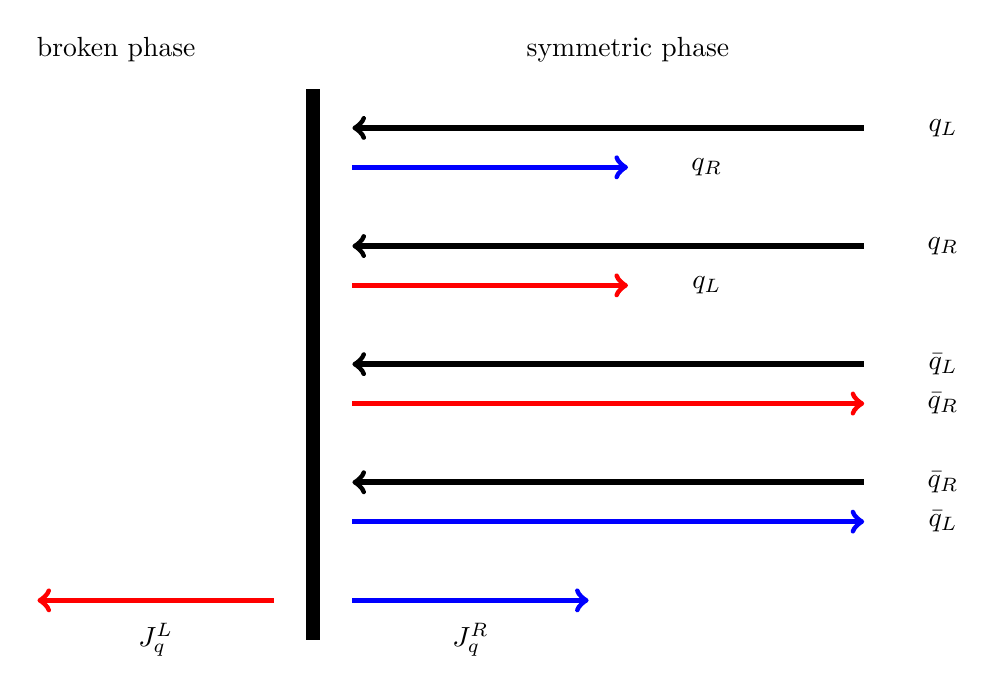
\begin{tikzpicture}
	\node at (-2.5,7) {broken phase};
	\node at (4,7) {symmetric phase};
	\draw [line width = 5pt](0,-.5) -- (0, 6.5);
	\draw [<-,line width = 2pt](.5,6)--(7,6);
	\node  at (8,6) {$q_L$};
	\draw [->,line width = 2pt,blue](.5,5.5)--(4,5.5);
	\node  at (5,5.5) {$q_R$};
	\draw [<-,line width = 2pt](.5,4.5)--(7,4.5);
	\node  at (8,4.5) {$q_R$};
	\draw [->,line width = 2pt,red](.5,4)--(4,4);
	\node  at (5,4) {$q_L$};
	\draw [<-,line width = 2pt](.5,3)--(7,3);
	\node  at (8,3) {$\bar{q}_L$};
	\draw [->,line width = 2pt,red](.5,2.5)--(7,2.5);
	\node  at (8,2.5) {$\bar{q}_R$};
	\draw [<-,line width = 2pt](.5,1.5)--(7,1.5);
	\node  at (8,1.5) {$\bar{q}_R$};
	\draw [->,line width = 2pt,blue](.5,1)--(7,1);
	\node  at (8,1) {$\bar{q}_L$};
	\draw [<-,line width = 2pt,red](-3.5,0)--(-.5,0);
	\node  at (-2,-.5) {$J_q^L$};
	\draw [->,line width = 2pt,blue](.5,0)--(3.5,0);
	\node  at (2,-.5) {$J_q^R$};
	
	\end{tikzpicture}
	\caption{Reflection of quarks and anti-quarks with different helicities respectively at a bubble wall. The length of the arrows of the reflected particles represents the flux of the respective particle. The effect of CP violation was chosen arbitrarily, by inverting it only the sings of the difference currents $J^L_q$ and $J^R_q$ would change but they would still cancel each other.}
	\label{fig:reflection}
\end{figure}
\subsection{Failures of the SM}
Since the SM offers everything needed to describe baryogenesis in the early universe, from B via C and CP violation to departures from the thermal equillibrium during the electroweak phase transition of possibly first order, one could naively say that the only thing left is the experimental proof to be delivered. \newline\indent
Having said this, recent experiments have shown that the SM alone, is not able to provide a strong enough phase transition of first order or more precisely a phase transition of first order at all. This will be shown in the following. \newline\indent
First, the reason why a strong first order transition is needed for baryogenesis is the following \cite[p. 25]{Bernreuther:2002uj}: Only for a strong first order phase transition the transition itself happens rapidly enough to keep up with the particle reactions and to induce a out-of-equilibrium state that way.\newline\indent
According to the Landau theory phase transitions are described by the behaviour of a order parameter. So for a first order phase transition the order parameter has to change dicontinuously at the critical point, while for a second order transition the order parameter has to change drastically as well, but this change occurs continuously. The way the order of the phase transition can be determinded is by introducing the order parameter as a new variable to the effective potential describing the free energy of the system which can be Taylor expanded with respect to the order parameter and temperature dependent coefficients in the vicinity of the phase transition, because here the order paramter ist small. The next step is to minimize the free energy with respect to the order parameter. If at some temperature the free energy shows to degenerated minima a first order phase transitions occurs because the transition from one minimum, or ground state, to another has to happen discontinously. If there are not more than one minima at a certain temperature but the ground state changes anyway a continuous phase transiton of higher order occured. 
\newline \indent
In a case of the electroweak phase transition the order parameter ist the expectation value of the Higgs field denoted as $v$ and the potential describes the energy of a system in a state with the Higgs expectation value $v$. Since in general this state is not one of minimal energy and because every system prefers to minimize its energy, it changes into a state described by the minimum of the potential where the expectation value of the Higgs is by definition the Higgs VEV. \newline\indent
As it is already known, the Higgs VEV had to change from zero at the big bang to a non-zero value while the universe cooled down to the temperature measured nowadays, so it is just natural to look at the change of this value with temperature. As discribed above, the change of the VEV can now happen continunously in which case the system undergoes a second order phase transition or discontinuously what is needed for a first order transition and especially for elektroweak baryogenesis. 
Both cases are shown in figure \ref{fig:higgs} for the effective Higgs potential
\begin{equation}
	V_\text{eff}=D(T^2-T_0)^2\phi^2-ET\phi^3-\frac{1}{4}\lambda\phi^4,
	\label{effective_pot}
\end{equation}
,including one-loop corrections \cite{Petropoulos:2003pm} for different non-zero temperature regimes. D and E are constant factors which are not relevant for this discussion and $\lambda$ describes the 4-Higgs self coupling.
\begin{figure}[H]
	\centering
	\begin{subfigure}{0.7\textwidth}
		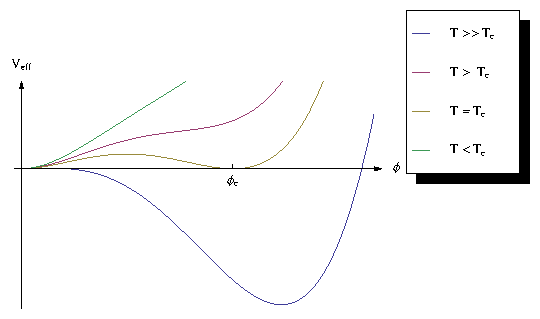
\includegraphics[width=\linewidth]{Images/Higgs1}
		\caption{Effective Higgs field for first order transition}
		\label{fig:higgs1}	
	\end{subfigure}
	\begin{subfigure}{0.7\textwidth}
		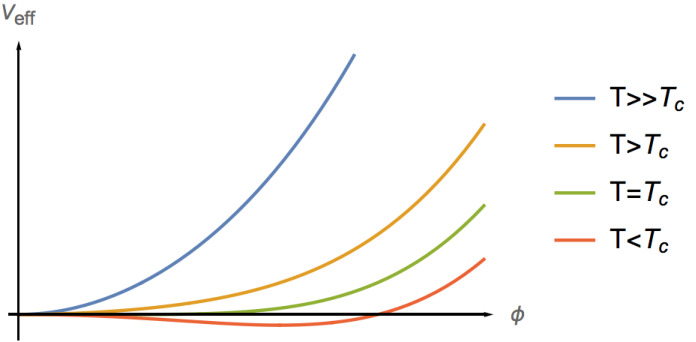
\includegraphics[width=\linewidth]{Images/Higgs2}
		\caption{Effective Higgs field for second order transition}
		\label{fig:higgs2}
	\end{subfigure}
	\caption{Effective Higgs field for different phase transitions}
	\label{fig:higgs}
\end{figure}
\noindent
Analyzing figure \ref{fig:higgs1} clearly shows the first order characteristics of the phase transition. While for high temperatures the VEV equals zero for the highly symmetric phase, the potential slowly develops a second minimum for decreasing temperature until at the critical temperature T=T$_c$ there are two energetically degenerated mimima, one at $\phi_1$=0 and one at $\phi_2$=$\phi_c$, which are separated by an energy barrier. However, the system can change from the minimum at $\phi_1$ to the one at $\phi_2$ via tunneling through the barrier resulting in a discontinuous change of the VEV and therefore inducing a first order phase transition. While the universe keeps on cooling down because of the universe's expanding, the new minimum gets energetically lowered while the original one stays at V$_\text{eff}$=0 and thus becomes a maximum, leaving an unstable state where once was a symmetric vacuum state. Since in both cases the new ground state does not have the same symmetry as original one, this phenomenon is called spontaneous symmetry breaking.\newline\indent
How this can be imagined in the early universe is that at some point in space and time the universe tunneled from one minimun to another thus breaking the symmetry locally and producing a local bubble of broken phase. These bubbles get bigger with time and combine with other bubbles whose generation gets much more likely as the lower temperatures lowers the barrier between the minima and increase the tunneling probability. \newline\indent
On the other hand, figure \ref{fig:higgs2} shows how the universe would develop in case of a second order transition. In this case even at T=T$_c$ there are no two degenerated minima but the new one develops gradually while the orignial minimum more and more becomes the unstable maximum you also get in figure \ref{fig:higgs1} for low temperatures. Since there are no two minima the universe can choose between, there is also no bubble formation but instead a continuous condensation throughout the universe which is not enough to induce baryogenesis. \newline\indent
Now that the two possibilities of the electroweak phase transition were represented the question how and why the SM fails to provide a strong enough first order phase transition still needs to be answered. \newline\indent
To do this it is useful to define a quantity that corresponds to the strenght of the phase transistion, which in this case will be 
\begin{equation}
	\frac{v_{T_c}}{T_c}\gtrsim1.
	\label{eq:strength_transition}
\end{equation}
The reason why \eqref{eq:strength_transition} is a good way to represent the strength of the phase transition is that by using equation \eqref{eq:spaleron} and the fact that the B+L violating sphaleron processes are exponentially surpressed by a Boltzmann factor inside of the phases with broken symmetry one gets for the rate of these spalerons at the critical temperature
\begin{equation}
	\Gamma_\text{sphaleron}\propto e^{-E_\text{sph}(T_c)/T_c}\propto e^{-v_{T_c}/T_c}.
	\label{eq:surpression}
\end{equation}
So equation \eqref{eq:surpression} really shows that the spaleron rates inside the bubbles with a Higgs VEV greater than zero are suppressed exactly by the quantity given in \eqref{eq:strength_transition}. So in order for these processes to be suppressed adequately has to be at least 1, which results in a suppression factor of roughly 0.36, for the phase transition to be strong enough to cause baryogenesis. \newline\indent 
There are various methods to use the condition in \eqref{eq:surpression} in order to calculate the Higgs mass and what the biggest mass is the Higgs particle can have in order for a first order phase transition to be possible which results in about m$_H$<70 GeV \cite[pp. 3f.]{Fodor:1999at}. \newline\indent
This theoretical result together with the experimental discovery that the Higgs mass is greater than 114 GeV \cite[pp. 100ff.]{Abbaneo:2001ix} clearly shows that the electroweak phase transition and therefore the SM as a whole is not able to explain how the observed baryonic asymmetry arose during the early times of the universe. \newline\indent
A solution for this problem is expanding the SM in such a way that the new elements are able to explain problems the SM was not able to. One of these expansions results in leptogenesis, what will be the topic of the following sections.